%%% LaTeX Template: Article/Thesis/etc. with colored headings and special fonts
%%%
%%% Source: http://www.howtotex.com/
%%% Feel free to distribute this template, but please keep to referal to http://www.howtotex.com/ here.
%%% February 2011
%%%
%%% Modified January 2016 by CDM

%%%  Preamble
\documentclass[11pt,letterpaper]{article}
\usepackage[margin=1.0in]{geometry}
\usepackage[T1]{fontenc}
\usepackage[bitstream-charter]{mathdesign}
\usepackage[latin1]{inputenc}					
\usepackage{amsmath}						
\usepackage{xcolor}
\usepackage{cite}
\usepackage{hyphenat}
\usepackage{graphicx}
\usepackage{float}
\usepackage{subfigure}
\usepackage{sectsty}
\usepackage[compact]{titlesec} 
\usepackage[tablegrid]{vhistory}
\usepackage{pbox}
\allsectionsfont{\color{accentcolor}\scshape\selectfont}

%%% Definitions
\definecolor{accentcolor}{rgb}{0.0,0.0,0.5} 
\newcommand{\teamname}{SegFault}
\newcommand{\productname}{Laser Harp}
\newcommand{\coursename}{CSE 4316: Senior Design I}
\newcommand{\semester}{Summer 2024}
\newcommand{\docname}{Project Charter}
\newcommand{\department}{Department of Computer Science \& Engineering}
\newcommand{\university}{The University of Texas at Arlington}
\newcommand{\authors}{Simon Aguirre \\ Matthew Moran \\ Thomas Pinkney \\ Alex Tran}

%%% Headers and footers
\usepackage{fancyhdr}
	\pagestyle{fancy}						% Enabling the custom headers/footers
\usepackage{lastpage}	
	% Header (empty)
	\lhead{}
	\chead{}
	\rhead{}
	% Footer
	\lfoot{\footnotesize \teamname \ - \semester}
	\cfoot{}
	\rfoot{\footnotesize page \thepage\ of \pageref{LastPage}}	% "Page 1 of 2"
	\renewcommand{\headrulewidth}{0.0pt}
	\renewcommand{\footrulewidth}{0.4pt}

%%% Change the abstract environment
\usepackage[runin]{abstract}			% runin option for a run-in title
%\setlength\absleftindent{30pt}			% left margin
%\setlength\absrightindent{30pt}		% right margin
\abslabeldelim{\quad}	
\setlength{\abstitleskip}{-10pt}
\renewcommand{\abstractname}{}
\renewcommand{\abstracttextfont}{\color{accentcolor} \small \slshape}	% slanted text

%%% Start of the document
\begin{document}

%%% Cover sheet
{\centering \huge \color{accentcolor} \sc \textbf{\department \\ \university} \par}
\vspace{1 in}
{\centering \huge \color{accentcolor} \sc \textbf{\docname \\ \coursename \\ \semester} \par}
\vspace{0.5 in}
\begin{figure}[h!]
	\centering
   	
\includegraphics[width=0.60\textwidth]{images/Logo}
\end{figure}
\vspace{0.5 in}
{\centering \huge \color{accentcolor} \sc \textbf{\teamname \\ \productname} \par}
\vspace{0.5 in}
{\centering \large \sc \textbf{\authors} \par}
\newpage


%\vspace{1 in}
%\centerline{January 13th, 2012}
%\newpage

%%% Revision History
\begin{versionhistory}
  	\vhEntry{1}{07.24.2024}{GH}{document creation}
\end{versionhistory}
\newpage

%%% Table of contents
\setcounter{tocdepth}{2}
\tableofcontents
\newpage

%%% List of figures and tables (optional)
\listoffigures
\listoftables
\newpage

%%% Document sections
\section{Introduction}
The laser harp is a novel musical instrument that utilizes laser beams to simulate the strings of a traditional harp. By interrupting these laser beams, users can produce corresponding musical notes, creating an engaging and interactive experience. This product is designed to be both educational and entertaining, aiming to inspire interest in STEM fields while providing a unique musical platform for enthusiasts and musicians.

\section{Product Concept}

The laser harp operates by projecting laser beams vertically from an array of laser emitters placed at the base. These beams are aligned with corresponding phototransistors positioned above, which detect the presence or absence of the laser light. When a user interrupts a laser beam by placing their hand in its path, the phototransistor detects the interruption and sends a signal to a microcontroller or a Raspberry Pi. The microcontroller processes this signal and triggers the playback of a pre-recorded musical note corresponding to the interrupted beam.

\section{Scope}

The scope of the laser harp project includes the design, development, and testing of a functional prototype that can demonstrate the key features and capabilities of the product. The project encompasses the following components:
\begin{itemize}
    \item \textbf{Laser and Phototransistor Array:} A set of laser emitters and phototransistors to detect beam interruptions.
    \item \textbf{Microcontroller/Raspberry Pi:} A processing unit to handle input signals from the phototransistors and control the audio output.
    \item \textbf{Audio System:} Speakers or an audio output interface to play the corresponding musical notes.
    \item \textbf{User Interface:} A simple and intuitive interface for calibration, instrument selection, pitch adjustment, octave control, and volume control.
    \item \textbf{Power Supply:} A reliable power source to ensure continuous operation of the laser harp.
\end{itemize}

\section{Key Requirements}

\begin{itemize}
    \item \textbf{Real-time Sound Playback:} The system must produce sound immediately upon the interruption of a laser beam, ensuring a responsive playing experience.
    \item \textbf{Multi-note Capability:} The laser harp should support the simultaneous interruption of multiple laser beams, allowing users to create chords.
    \item \textbf{User Interface:} A user-friendly interface for controlling various parameters such as instrument selection, pitch, octave, and volume.
    \item \textbf{Portability:} The device should be lightweight and easy to transport, making it suitable for demonstrations and performances in different locations.
    \item \textbf{Safety:} The lasers used must be Class 1 to ensure user safety, with no risk of direct eye exposure.
    \item \textbf{Power Supply:} The system should be powered by a reliable source, such as a rechargeable battery or an external power adapter, to ensure uninterrupted operation.
    \item \textbf{Durability:} The construction of the laser harp should be robust enough to withstand regular use and transportation.
\end{itemize}

By addressing these key requirements, the architectural design of the laser harp will focus on creating a functional, safe, and user-friendly musical instrument that can be used for both educational purposes and entertainment. The following sections will detail the specific design components, their interactions, and the overall system architecture to achieve the desired functionality and performance.

\newpage
\section{System Overview}
Explain, at a high level, how you will implement a solution to the problem. Include a diagram of major components to the system (not a full architectural design, but a high level overview of the major system components and how a user or external system might interface). Avoid specific implementation details (operating system, programming languages, etc.). This section should occupy at least 1 full page.
\newpage
\section{Subsystem Definitions \& Data Flow}
This section breaks down your layer abstraction to another level of detail. Here you grapically represent the logical subsytems that compose each layer and show the interactions/interfaces between those subsystems. A subsystem can be thought of as a programming unit that implements one of the major functions of the layer. It, therefore, has data elements that serve as source/sinks for other subsystems. The logical data elements that flow between subsystems need to be explicitly defined at this point, beginning with a data flow-like diagram based on the block diagram.

\begin{figure}[h!]
	\centering
 	\includegraphics[width=\textwidth]{images/Subsystem}
 \caption{A simple data flow diagram}
\end{figure}

\newpage
\section{Input Layer Subsystems}
The input layer is a layer that allows users of the harp to interact with the hardware itself so it may play noises or change the corresponding noises that may play while displaying a visual on the touch screen

\subsection{Laser Diodes Subsystem}
The laser Diode subsystem is a hardware component in which the user can interact with the lasers, when the lasers are interacted with the software will decide what laser has been interacted with and create a noise through the sound multiplexer


\begin{figure}[h!]
	\centering
 	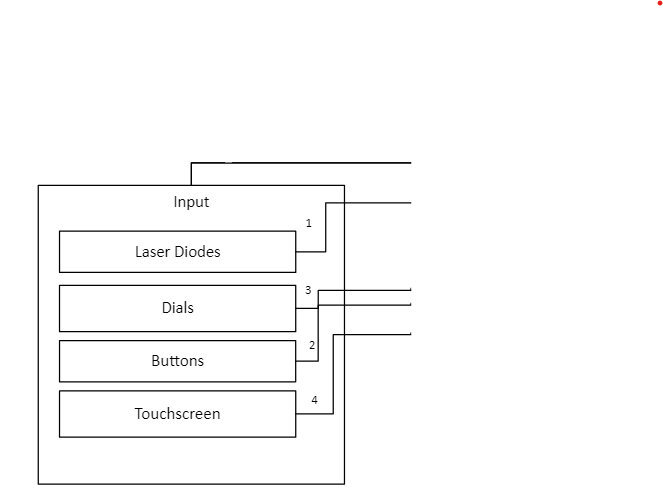
\includegraphics[width=0.60\textwidth]{images/InputSubsystem}
 \caption{Laser Diodes Subsystem}
\end{figure}

\subsubsection{Assumptions}
It is assumed that the laser system will be used in a proper way by breaking the contact of the laser diode and photo transistor

\subsubsection{Responsibilities}
Interacted by the user in order to interact with the control unit subsection in order to make noise


\subsubsection{Subsystem Interfaces}

\begin {table}[H]
\caption {Subsystem interfaces} 
\begin{center}
    \begin{tabular}{|  p{1cm}  |p{6cm}  |p{3cm}  |p{3cm} |}
    \hline
    ID & Description & Inputs & Outputs \\ \hline
    \#1& Powers a Laser Diode wich can be interacted with& User Input& \pbox{3cm}{Sound Multiplexer}\\\hline
    \end{tabular}
\end{center}
\end{table}




\subsection{Dials Subsystem}
The Dials are a subsystem which interacts with the Control unit in order to change octaves are instruments which can be selected


\begin{figure}[h!]
	\centering
 	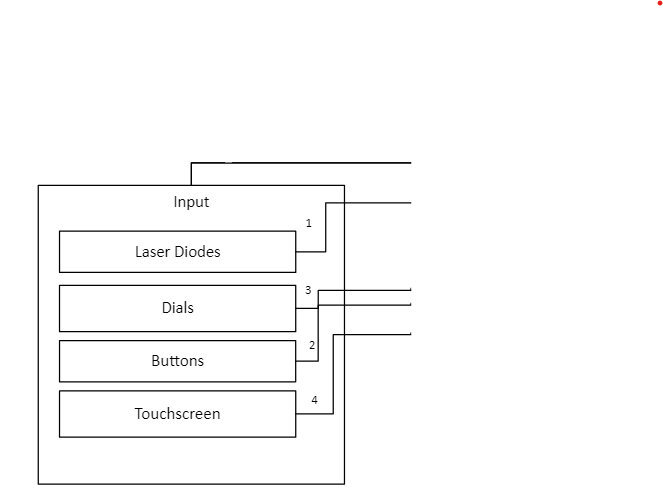
\includegraphics[width=0.60\textwidth]{images/InputSubsystem}
 \caption{Dials}
\end{figure}

\subsubsection{Assumptions}
 Dials should be rotated in a horizontal movement in order for the system to register input


\subsubsection{Responsibilities}
Dials will be used to control the sound setting which can be used to turn up or turn down the sound of the harp through the speakers

\subsubsection{Subsystem Interfaces}

\begin {table}[H]
\caption {Subsystem interfaces} 
\begin{center}
    \begin{tabular}{|  p{1cm}  |p{6cm}  |p{3cm}  |p{3cm} |}
    \hline
    ID & Description & Inputs & Outputs \\ \hline
    \#1& Used to adjust the sound setting & Human input& \pbox{3cm}{Speaker}\\\hline
    \end{tabular}
\end{center}
\end{table}



\subsection{Buttons Subsystem}
Buttons are used to change octaves or interact with different areas of the control unit.

\begin{figure}[h!]
	\centering
 	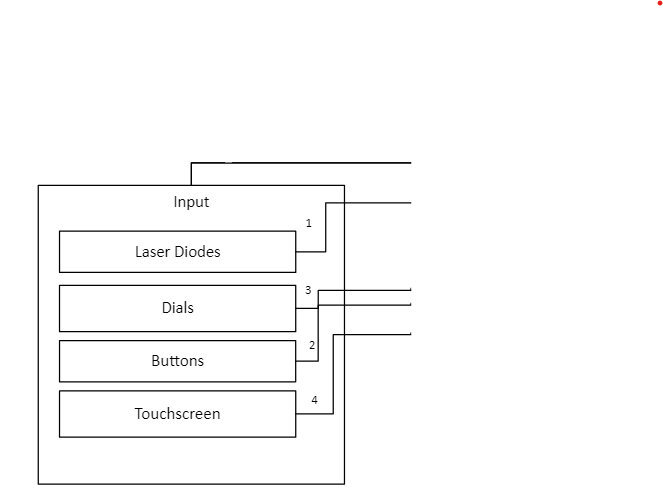
\includegraphics[width=0.60\textwidth]{images/InputSubsystem}
 \caption{Buttons}
\end{figure}

\subsubsection{Assumptions}
A assumption to be made for the buttons is that they are used as a alternative way as a input for the control unit


\subsubsection{Responsibilities}
The responsibility of the button is to control the sound settings and interact with the sound settings such as lowering the volume and the user settings such as changing octave or instruments 


\subsubsection{Subsystem Interfaces}

\begin {table}[H]
\caption {Subsystem interfaces} 
\begin{center}
    \begin{tabular}{|  p{1cm}  |p{6cm}  |p{3cm}  |p{4cm}|}
    \hline
    ID & Description & Inputs & Outputs \\ \hline
    \#1& Round buttons which may be pressed in order to change sound levels or instruments& User input&       Sound Settings and user Settings\\\hline
    \end{tabular}
\end{center}
\end{table}

\subsection{Touchscreen Subsystem}
The touchscreen is used for visual display and to display certain elements of settings to the user, the touchscreen can be used as a alternative way to interact with the control unit


\begin{figure}[h!]
	\centering
 	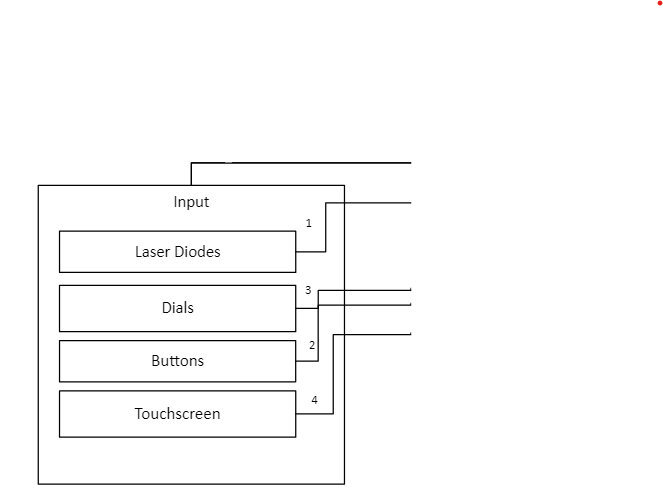
\includegraphics[width=0.60\textwidth]{images/InputSubsystem}
 \caption{Touchscreen}
\end{figure}

\subsubsection{Assumptions}
The touchscreen should be used as the primary way to interact with the control unit


\subsubsection{Responsibilities}
The touch screen main responsibility is to function as a visual output and as a way to interact with the OS and program which will have the user settings and sound settings


\subsubsection{Subsystem Interfaces}

\begin {table}[H]
\caption {Subsystem interfaces} 
\begin{center}
    \begin{tabular}{|  p{1cm}  |p{6cm}  |p{3cm}  |p{3cm} |}
    \hline
    ID & Description & Inputs & Outputs \\ \hline
    \#1& Takes input from the user by pressing on the screen also displays visuals& User input& \pbox{3cm}{UserSettings}\pbox{3cm}{Sound Settings}\\\hline
    \end{tabular}
\end{center}
\end{table}


\newpage
\section{Control Unit Layer Subsystems}
This section describes the Control Unit layer, responsible for processing input data, managing system logic, and generating output signals.
\begin{figure}[h!]
	\centering
 	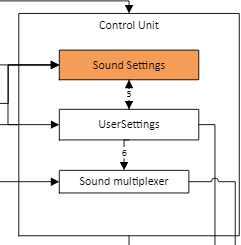
\includegraphics[width=0.60\textwidth]{images/SoundSettings.png}
 \caption{Sound Settings subsystem description diagram}
\end{figure}
\subsection{Sound setting}
This section describes the Control Unit layer, responsible for processing input data, managing system logic, and generating output signals.


\subsubsection{Assumptions}
The Sound Settings subsystem receives digital signals from the UserSettings and the Sound Settings subsystem is responsible for managing and applying the sound settings based on user input.

\subsubsection{Responsibilities}
\begin{itemize}
\begin{item}
Receive digital signals from the UserSettings subsystem representing the user's desired sound settings.
\end{item}
\begin{item}
Process and store the received sound settings. 
\end{item}
\begin{item}
Generate digital signals representing the selected sound settings to the Sound Multiplexer subsystem 
\end{item}
\end{itemize}

\subsubsection{Subsystem Interfaces}

\begin {table}[H]
\caption {Subsystem interfaces} 
\begin{center}
    \begin{tabular}{ | p{1cm} | p{6cm} | p{3cm} | p{3cm} |}
    \hline
    ID & Description & Inputs & Outputs \\ \hline
    \#1 & Receive digital signal from the UserSetting  & \pbox{3cm}{ \\ User settings and input } & \pbox{3cm}{User setting}  \\ \hline
 
    \end{tabular}
\end{center}
\end{table}

\subsection{UserSettings}
The UserSettings subsystem is connected to the Sound Settings and the Sound Multiplexer subsystem
\begin{figure}[h!]
	\centering
 	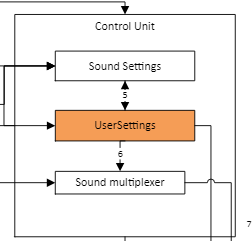
\includegraphics[width=0.60\textwidth]{images/UserSettings}
 \caption{User Settings subsystem description diagram}
\end{figure}


\subsubsection{Assumptions}
\begin{itemize}
\begin{item}
The UserSettings subsystem receives digital signals from the Sound Settings subsystem 
\end{item}
\begin{item}
The UserSettings subsystem can receive user input from the Input Layer subsystems
\end{item}
\begin{item}
The UserSettings subsystem is responsible for managing and updating the user's settings
\end{item}
\end{itemize}
\subsubsection{Responsibilities}
\begin{itemize}
\begin{item}
Receive user input from the Input Layer subsystems.
\end{item}
\begin{item}
Process and validate user input.
\end{item}
\begin{item}
Update the user's settings based on the validated input.
\end{item}
\begin{item}
Send digital signals representing the user's settings to the Sound Settings subsystem
\end{item}
\end{itemize}

\subsubsection{Subsystem Interfaces}
\begin {table}[H]
\caption {Subsystem interfaces} 
\begin{center}
    \begin{tabular}{ | p{1cm} | p{6cm} | p{3cm} | p{3cm} |}
    \hline
    ID & Description & Inputs & Outputs \\ \hline
    \#1 & Receives digital signals from the Sound Settings & \pbox{3cm}{ \\ Digital signals representing sound settings } & \pbox{3cm}{Touchscreen}  \\ \hline
    
    \end{tabular}
\end{center}
\end{table}
\subsection{Sound multiplexer}
The Sound Multiplexer subsystem is connected to the Sound Settings subsystem and the Output Layer
\begin{figure}[h!]
	\centering
 	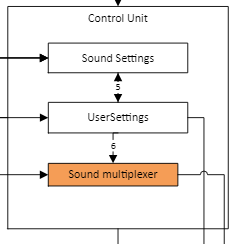
\includegraphics[width=0.60\textwidth]{images/Soundmultiplex}
 \caption{Sound Multiplexer subsystem description diagram}
\end{figure}


\subsubsection{ASSUMPTIONS}
\begin{itemize}
\begin{item}
The Sound Multiplexer subsystem receives digital signals from the Sound Settings subsystem 
\end{item}
\begin{item}
The Sound Multiplexer subsystem can select and output the appropriate sound based on the received settings.
\end{item}
\begin{item}
The Sound Multiplexer subsystem is responsible for managing and outputting the final sound signal.
\end{item}
\end{itemize}
\subsubsection{SUBSYSTEM INTERFACES}
\begin {table}[H]
\caption {Subsystem interfaces} 
\begin{center}
    \begin{tabular}{ | p{1cm} | p{6cm} | p{3cm} | p{3cm} |}
    \hline
    ID & Description & Inputs & Outputs \\ \hline
    \#1 & Representing the desired sound settings from the Sound Settings subsystem & \pbox{3cm}{ \\ User settings and input } & \pbox{3cm}{Speaker}  \\ \hline
  
    \end{tabular}
\end{center}
\end{table}
\newpage
\section{Output Layer Subsystems}
In this section, the layer is described in some detail in terms of its specific subsystems. Describe each of the layers and its subsystems in a separate chapter/major subsection of this document. The content of each subsystem description should be similar. Include in this section any special considerations and/or trade-offs considered for the approach you have chosen.

\subsection{Subsystem 1}
This section should be a general description of a particular subsystem for the given layer. For most subsystems, an extract of the architectural block diagram with data flows is useful. This should consist of the subsystem being described and those subsystems with which it communicates.

\begin{figure}[h!]
	\centering
 	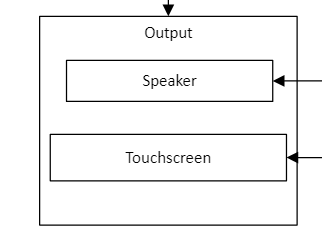
\includegraphics[width=0.60\textwidth]{images/OutputSubsystem}
 \caption{Example subsystem description diagram}
\end{figure}

\subsubsection{Assumptions}
Any assumptions made in the definition of the subsystem should be listed and described. Pay particular attention to assumptions concerning interfaces and interactions with other layers.

\subsubsection{Responsibilities}
Each of the responsibilities/features/functions/services of the subsystem as identified in the architectural summary must be expanded to more detailed responsibilities. These responsibilities form the basis for the identification of the finer-grained responsibilities of the layer's internal subsystems. Clearly describe what each subsystem does.

\subsubsection{Subsystem Interfaces}
Each of the inputs and outputs for the subsystem are defined here. Create a table with an entry for each labelled interface that connects to this subsystem. For each entry, describe any incoming and outgoing data elements will pass through this interface.

\begin {table}[H]
\caption {Subsystem interfaces} 
\begin{center}
    \begin{tabular}{ | p{1cm} | p{6cm} | p{3cm} | p{3cm} |}
    \hline
    ID & Description & Inputs & Outputs \\ \hline
    \#xx & Description of the interface/bus & \pbox{3cm}{input 1 \\ input 2} & \pbox{3cm}{output 1}  \\ \hline
    \#xx & Description of the interface/bus & \pbox{3cm}{N/A} & \pbox{3cm}{output 1}  \\ \hline
    \end{tabular}
\end{center}
\end{table}

\subsection{Subsystem 2}
Repeat for each subsystem

\subsection{Subsystem 3}
Repeat for each subsystem

\newpage

%%% References
\bibliographystyle{plain}
\bibliographystyle{reference/IEEEtran_custom}
\bibliography{reference/refs}{}

\end{document}
